As said before the software is still in it early stages, as it's an MVP and some
functionalities are still just a proof of concept. And it's following the architecture
in the figure \ref{fig:entities_cd}.

\begin{figure}[!ht]
    \centering
    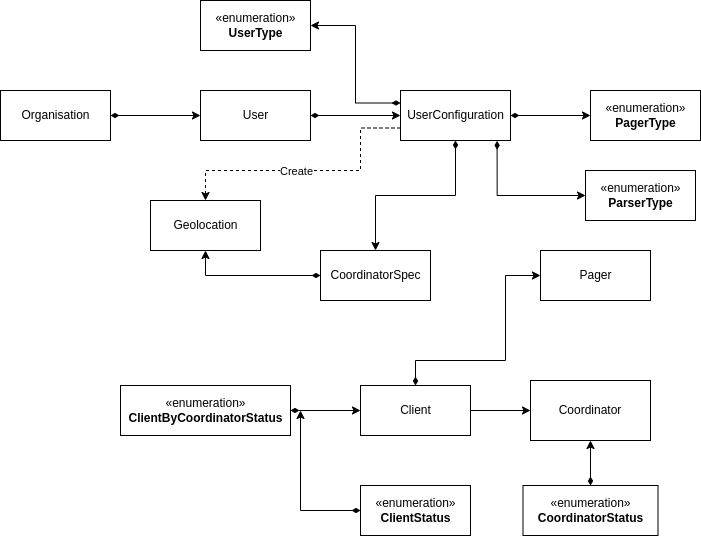
\includegraphics[width=1\textwidth]{images/Conceptual Model.png}
    \caption{\footnotesize{Business logic - Class diagram}}
    \label{fig:entities_cd}
\end{figure}

Which constitutes the entities of the software, and they are:

\begin{itemize}
    \item User: represents a Site\footnote{Site represents the factory
        or warehouse which is being managed} not an actual human user
        which comes with it limitations when it comes to having mulitple
        actors within a site to manage the multiple available flows for
        each user, which would require a permissions system.
    \item UserConfiguration: it's a configuration for the site, which
        can set the parameters that are specific to the site,
        like the name of the site, specfic documents for the management,
        the docks that it has, geolocation of the docks, \dots
    \item Coordinator: It's the entity representative of the docks.
    \item PagerType: Is representative of types of devices that can
        be used to send messages to the user.
    \item Client: the entity that is in this case represents the driver,
        used to take care of geolocating them, loading their files,
        giving them access to the platform, \dots.
\end{itemize}

The rest of the classes are pretty self explanatory. And those entities are 
connected to each other either by direct aggregation or by composition, or
some get the relationship later on within the services to have the dependencies
within fulfill.

The backend is done in a pure microservice architecture as shown in figure
\ref{fig:microservices_spring}. Meaning that the services are all microservices,
and the communication inside of the Spring application is done through function
calls between different layers.

\begin{figure}[!ht]
    \centering
    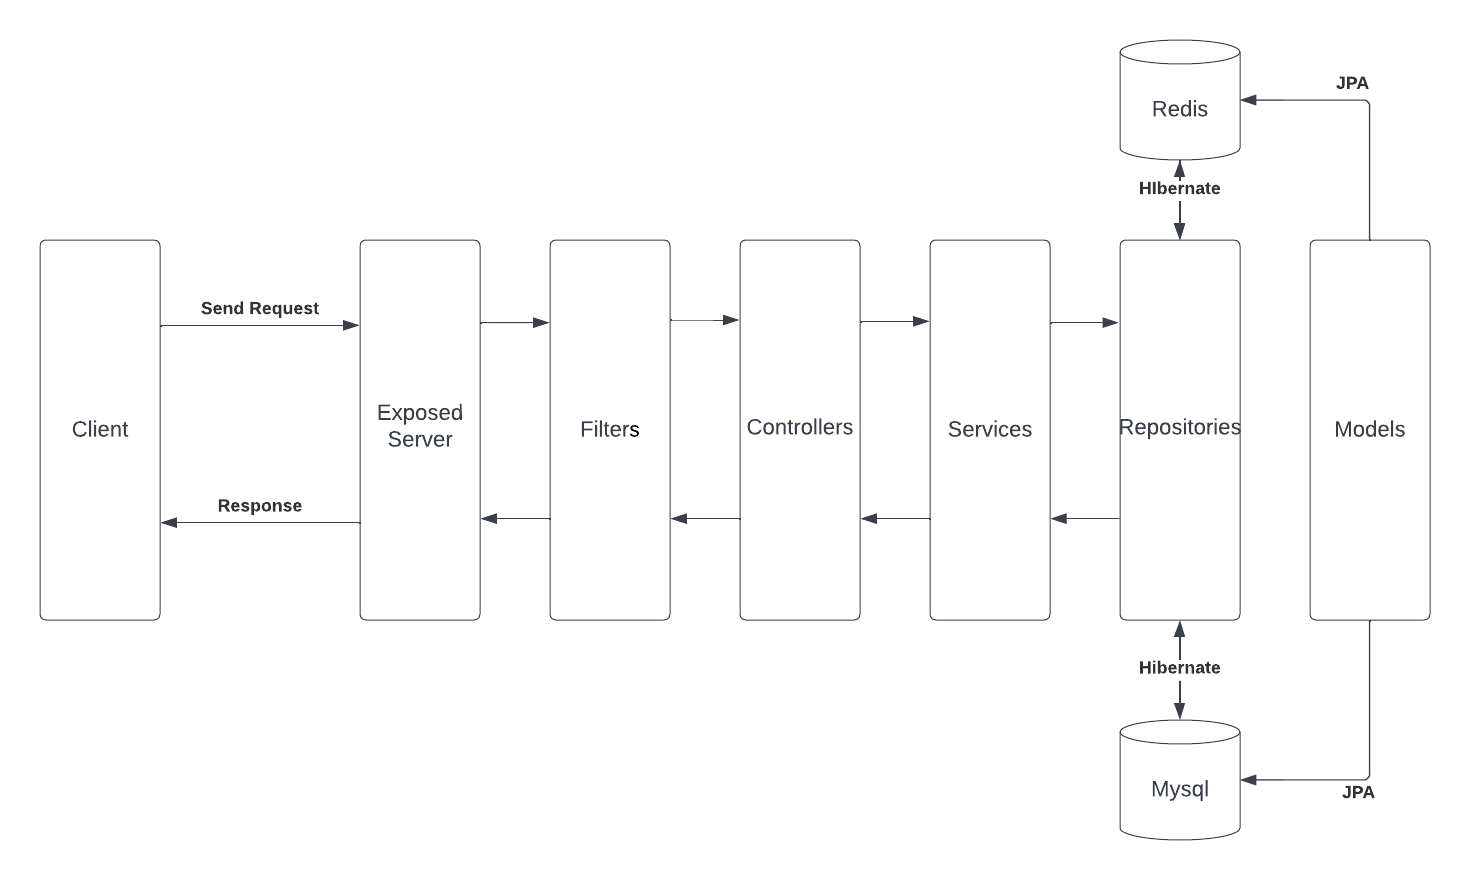
\includegraphics[width=1\textwidth]{images/Microservices Spring.png}
    \caption{\footnotesize{Current Spring Microservices Architecture}}
    \label{fig:microservices_spring}
\end{figure}

The layers that are in talk are:

    \begin{itemize}
        \item \textbf{Entities Layer}: 
            It's the layer that contains the entities and their relationships,
            which are shown in the figure \ref{fig:entities_cd}.
        \item \textbf{Persistence Layer}:
            This is mainly for the data handling, CRUD operations and operating
            sessions with the database.
        \item \textbf{Service Layer}:
            This layer is the one where business logic is implemented,
            containing everything from calling talking to the database,
            to processing it to be returned to the client.
        \item \textbf{Controller Layer}:
            This is where the handling of the requests is done to pipe them
            to the service layer.
        \item \textbf{Filter Layer}:
            Before any request achieving the controllers, it's first handled by
            the filter layer which stands on the API Gateway level and is
            responsible for the authorization of the request.
        \item \textbf{Gateway Layer}:
            This is the layer that is responsible for the communication between
            the microservices, and the client.
    \end{itemize}

And those layers constitute the main aspects of how the software is structured in
a zoomed out approach.

The development approach that they went with is the Reactive Paradigm in combination
with OOP. The Reactive Paradigm is a general approach to the programming, which is focused 
on reacting to changes, such as data values or events, a simple example could be spreadsheets
cells that are constantly updated, when data is update on a different cell, meaning the 
cell reacted to the change of the other cell \cite{reactive_programming}.
The Reactive approach is clearly advantageous in terms of performance in the system
that they are building as there is constant communication between the microservices,
real-time data getting processed and websockets being used for communication.

Finally the Java Spring backend is handled by the build tool Gradle, which is a
Java build automation tool focused on improving the build process, it allows to be scripted
using either a Groovy or Kotlin DSL \cite{gradle_def}.
This tool allows for the building, launching and testing, but most importantly importing 
the dependencies of the project.

Finally the deployment was taking multiple steps, the first one related to the backend
and the second one related to the frontend. The first one was to build the application
using the Gradle build tool and then deploying it to the AWS EC2 instance using the 
SCP protocol, once build is on the EC2 instance, the next move was to SSH into the 
instance and restart the application. The second one was to build the frontend using
the angular CLI tool, and then deploying the front end part to the AWS S3 bucket,
which hosted the front end part of the application.

